\chapter{Week 1: Lab Methods and Organelles}\label{Week 1: Lab Methods and Organelles}

\section{Background}\label{Background}
\begin{itemize}
  \item \jjj{Describe The steps in Tissue Preparation for microscopy:}
    \begin{itemize}
      \item Fixation:
      \item Embedding:
      \item Staining:
    \end{itemize}
  \item \jjj{What does H \& E Stain?}
  \item \jjj{What does PAS Stain?}
  \item \jjj{Describe Enzyme Histochemistry.}
  \item \jjj{How does Immunohistochemistry work?}
\end{itemize}

\section{Microscopic Techniques}
\begin{itemize}
  \item \jjj{Bright field}:
  \item \jjj{Phase contrast}:
  \item \jjj{Confocal}:
  \item \jjj{Fluorescent}:
  \item \jjj{Scanning Electron Microscopy}:
  \item \jjj{Transmission Electron Microscopy}:
\end{itemize}

\section{Organelles and Cytoplasmic Inclusions}
\begin{itemize}
  \item \jjj{Nucleolus}
  \begin{itemize}
    \item Structure:
    \item Size:
    \item Light Microscopic Features:
    \item Function:
  \end{itemize}
  \item \jjj{Plasma Membrane}
  \begin{itemize}
    \item Structure:
    \item Size:
    \item Light Microscopic Features:
    \item Function:
  \end{itemize}
  \item \jjj{rER}
  \begin{itemize}
    \item Structure:
    \item Size:
    \item Light Microscopic Features:
    \item Function:
  \end{itemize}
  \item \jjj{sER}
  \begin{itemize}
    \item Structure:
    \item Size:
    \item Light Microscopic Features:
    \item Function:
  \end{itemize}
  \item \jjj{Golgi Apparatus}
  \begin{itemize}
    \item Structure:
    \item Size:
    \item Light Microscopic Features:
    \item Function:
  \end{itemize}
  \item \jjj{Secretory Vesicles}
  \begin{itemize}
    \item Structure:
    \item Size:
    \item Light Microscopic Features:
    \item Function:
  \end{itemize}
  \item \jjj{Mitochondria}
  \begin{itemize}
    \item Structure:
    \item Size:
    \item Light Microscopic Features:
    \item Function:
  \end{itemize}
  \item \jjj{Endosomes}
  \begin{itemize}
    \item Structure:
    \item Size:
    \item Light Microscopic Features:
    \item Function:
  \end{itemize}
  \item \jjj{Lysosomes}
  \begin{itemize}
    \item Structure:
    \item Size:
    \item Light Microscopic Features:
    \item Function:
  \end{itemize}
  \item \jjj{Peroxisomes}
  \begin{itemize}
    \item Structure:
    \item Size:
    \item Light Microscopic Features:
    \item Function:
  \end{itemize}
  \item \jjj{Cytoskeletal Elements}
  \begin{itemize}
    \item Structure:
    \item Size:
    \item Light Microscopic Features:
    \item Function:
  \end{itemize}
  \item \jjj{Ribosomes}
  \begin{itemize}
    \item Structure:
    \item Size:
    \item Light Microscopic Features:
    \item Function:
  \end{itemize}
  \item \jjj{Glycogen}
  \begin{itemize}
    \item Structure:
    \item Size:
    \item Light Microscopic Features:
    \item Function:
  \end{itemize}
  \item \jjj{Lipid Droplets}
  \begin{itemize}
    \item Structure:
    \item Size:
    \item Light Microscopic Features:
    \item Function:
  \end{itemize}

  \subsection{Labeled Organelle Diagram}
  \begin{itemize}
    \item 
  \end{itemize}
\end{itemize}

  \section{Mitotic Phases}
  \begin{center}
    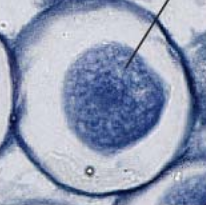
\includegraphics[scale=0.5]{images/week-1-mp1.png}
  \end{center}
  \begin{itemize}
    \item 
  \end{itemize}
  \begin{center}
    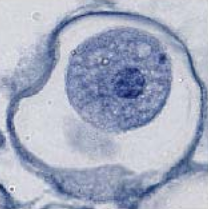
\includegraphics[scale=0.5]{images/week-1-mp2.png}
  \end{center}
  \begin{itemize}
    \item 
  \end{itemize}
  \begin{center}
    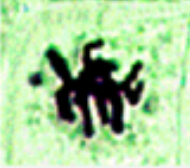
\includegraphics[scale=0.5]{images/week-1-mp3.png}
  \end{center}
  \begin{itemize}
    \item 
  \end{itemize}
  \begin{center}
    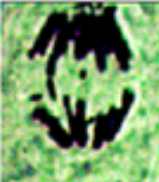
\includegraphics[scale=0.5]{images/week-1-mp4.png}
  \end{center}
  \begin{itemize}
    \item 
  \end{itemize}
  \begin{center}
    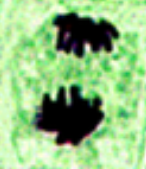
\includegraphics[scale=0.5]{images/week-1-mp5.png}
  \end{center}
  \begin{itemize}
    \item 
  \end{itemize}

  
\section{Apoptosis Events}\label{Apoptosis Events}
\begin{itemize}
  \item \jjj{DNA fragmentation}:
  \item \jjj{Decrease of cell volume}:
  \item \jjj{Membrane Blebbing}:
  \item \jjj{Formation of apoptotic bodies}:
\end{itemize}

\section{Features and Functions}
\begin{itemize}
  \item \jjj{Stratified squamous epithelium}:
  \begin{itemize}
    \item Features:
    \item Functions:
  \end{itemize}
  \item \jjj{Simple cuboidal epithelium}:
  \begin{itemize}
    \item Features:
    \item Functions:
  \end{itemize}
  \item \jjj{Skeletal muscle}:
  \begin{itemize}
    \item Features:
    \item Functions:
  \end{itemize}
  \item \jjj{Cardiac muscle}:
  \begin{itemize}
    \item Features:
    \item Functions:
  \end{itemize}
  \item \jjj{Smooth muscle}:
  \begin{itemize}
    \item Features:
    \item Functions:
  \end{itemize}
\end{itemize}